\begin{frame}{What SLAM Solves}
  \begin{itemize}\footnotesize\itemsep0.3em
    \item \textbf{SLAM, stated formally} (Cadena et al.): ``SLAM comprises the simultaneous estimation of the state of a robot equipped with on-board sensors, and the construction of a model (the map) of the environment that the sensors are perceiving.'' In visual SLAM the state is the camera pose $T_t\in SE(3)$ at each time $t$.
    \item \textbf{Chicken and egg:} tracking the pose needs a map to register each frame against, and building the map needs the poses that triangulate it, so both are estimated together.
    \item \textbf{Online and causal:} the estimate at time $t$ uses only frames up to $t$ and must keep pace with the camera.
  \end{itemize}
  \vspace{0.1em}
  {\centering\scriptsize
  \begin{tabular}{>{\raggedright\arraybackslash}p{1.8cm} >{\raggedright\arraybackslash}p{2.7cm} >{\raggedright\arraybackslash}p{2.8cm} >{\raggedright\arraybackslash}p{4.5cm}}
    \toprule
     & \textbf{Visual odometry (VO)} & \textbf{Visual SLAM} & \textbf{SfM} \\
    \midrule
    Input & ordered video stream & ordered video stream & unordered image set \\
    \addlinespace[0.1em]
    Processing & online, causal & online, causal & offline, all images available from the start \\
    \addlinespace[0.1em]
    Revisited places & not recognized: the world looks like an ``infinite corridor'' & recognized by loop closure, so the map keeps the true topology & matched like any other overlapping pair \\
    \addlinespace[0.1em]
    Error over time & drift grows without bound & reset at each loop closure & no time order; incremental SfM drifts along the registration order, which global bundle adjustment (BA) corrects \\
    \bottomrule
  \end{tabular}\par}
  \vspace{0.3em}
  {\scriptsize Cadena et al., ``Past, Present, and Future of Simultaneous Localization And Mapping: Towards the Robust-Perception Age,'' IEEE T-RO 2016, \href{https://arxiv.org/abs/1606.05830v4}{arXiv:1606.05830v4}, Sec.~I.\par}
\end{frame}

\begin{frame}{Anatomy of a Visual SLAM System}
  \begin{itemize}\scriptsize\itemsep0.3em
    \item ``The front-end abstracts sensor data into models that are amenable for estimation, while the back-end performs inference on the abstracted data produced by the front-end'' (Cadena et al., Sec.~II).
  \end{itemize}
  \vspace{0.1em}
  {\centering
  \begin{tikzpicture}[font=\sffamily\scriptsize, >=latex,
      blk/.style={draw, rounded corners=2pt, align=center, minimum height=0.72cm, inner sep=2pt},
      fe/.style={blk, fill=blue!12}, be/.style={blk, fill=orange!16}, mp/.style={blk, fill=green!14}]
    \node[blk, fill=gray!10] (cam) at (0,1.85) {Camera\\frames};
    \node[fe] (feat) at (2.3,1.85) {Features,\\short-term matching};
    \node[fe] (pose) at (5.2,1.85) {Pose tracking\\(PnP, local map)};
    \node[fe, diamond, aspect=1.7, inner sep=0.5pt] (kf) at (7.7,1.85) {Key-\\frame?};
    \node[be] (lba) at (10.4,1.85) {Local BA\\(window of keyframes)};
    \node[fe] (reloc) at (1.6,0.4) {Relocalization\\(retrieve, PnP)};
    \node[mp] (map) at (5.9,0.4) {Map: keyframes,\\points, covisibility};
    \node[fe] (loop) at (9.2,0.4) {Loop detection\\(retrieve, RANSAC)};
    \node[be] (pgo) at (12.15,0.4) {Pose-graph\\optimization};
    \draw[->] (cam) -- (feat);
    \draw[->] (feat) -- (pose);
    \draw[->] (pose) -- (kf);
    \draw[->] (kf) -- node[above] {yes} (lba);
    \draw[->] (lba.south) -- node[left=1pt, pos=0.62] {keyframe} (loop.north);
    \draw[->] (lba.south west) -- node[left=2pt, pos=0.45] {new points} (map.north east);
    \draw[->] (loop) -- node[above, align=center] {loop\\edge} (pgo);
    \draw[->] (pgo.south) -- ++(0,-0.35) -| node[pos=0.25, below] {corrected poses and points} (map.south);
    \draw[->] (map.north -| pose.south) -- node[right] {local map} (pose.south);
    \draw[<->] (pose.south west) -- node[left=2pt] {if lost} (reloc.north east);
    \draw[->] (map) -- node[above] {keyframes} (reloc);
  \end{tikzpicture}\par}
  \vspace{0.1em}
  {\centering\scriptsize Blue: front-end (data association); orange: back-end (estimation); green: the map that both read and write.\par}
  \vspace{0.1em}
  \begin{columns}[T,onlytextwidth]
    \column{0.48\textwidth}
      \begin{itemize}\scriptsize\itemsep0.2em
        \item \textbf{Front-end:} data association (deciding which measurements show the same 3D point): extract features (ORB), match them to the local map, and estimate the pose from these 2D--3D matches (PnP), refined by motion-only BA (points fixed).
        \item \textbf{Keyframes:} only frames that add new views enter the back-end. BA cost grows with the number of keyframes, so redundant ones are culled.
      \end{itemize}
    \column{0.50\textwidth}
      \begin{itemize}\scriptsize\itemsep0.2em
        \item \textbf{Back-end:} local BA over nearby keyframes (covisible, i.e.\ sharing map points, or recent); after a loop closure, a pose graph: all keyframe poses, linked by relative-pose edges.
        \item \textbf{Relocalization:} when tracking fails, retrieve similar keyframes and solve PnP in RANSAC; loop detection is the same long-term data association.
      \end{itemize}
  \end{columns}
\end{frame}

\begin{frame}{Drift and Loop Closure}
  \begin{columns}[T,onlytextwidth]
    \column{0.65\textwidth}
      \begin{itemize}\scriptsize\itemsep0.15em
        \item \textbf{Drift:} each relative pose carries a small error, and chaining them makes the error grow without bound. One camera cannot observe scale, so the map drifts in all 7 gauge DoF: rotation, translation and scale.
        \item \textbf{Detect the revisit} (place recognition): image retrieval with global descriptors and approximate nearest-neighbour search, or a \textbf{bag of binary words}. DBoW2 quantizes BRIEF descriptors (the descriptor inside ORB) with a vocabulary tree (hierarchical k-medians clustering, 10 branches, 6 levels; its $10^6$ leaves are the words), so an image becomes a histogram of words, weighted by tf-idf (term frequency times inverse document frequency: words rare across images count more). An inverted index (each word's list of images) returns the candidates.
        \item \textbf{Verify:} RANSAC on a fundamental matrix with at least 12 inliers (DBoW2), or on a 3D-to-3D similarity (ORB-SLAM, next slide).
        \item \textbf{Correct:} add the loop edge and optimize a pose graph over similarities $S=\left[\begin{smallmatrix} sR & \mathbf{t}\\ \mathbf{0}^\top & 1\end{smallmatrix}\right]\in\mathrm{Sim}(3)$ with scale $s>0$:
        \[ \min_{\{S_i\}} \sum_{(i,j)\in\mathcal{E}} \mathbf{e}_{ij}^\top \Lambda_{ij}\,\mathbf{e}_{ij},\quad \mathbf{e}_{ij}=\log_{\mathrm{Sim}(3)}\!\big(S_{ij}S_jS_i^{-1}\big)\in\mathbb{R}^7 \]
        $S_i$: world-to-keyframe similarity; $S_{ij}$: measured relative similarity (odometry or loop edge); $\log$: the 7-vector of rotation, translation and log-scale; $\Lambda_{ij}$: information matrix, the inverse covariance of the edge (identity in ORB-SLAM); one keyframe is held fixed to remove the 7 gauge DoF.
      \end{itemize}
    \column{0.33\textwidth}
      \centering
      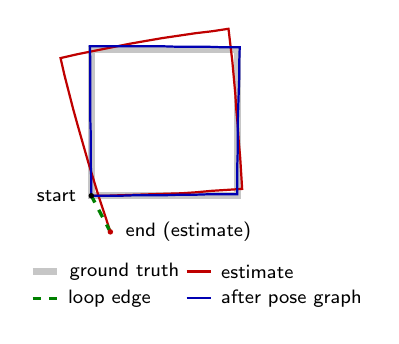
\begin{tikzpicture}[font=\sffamily\scriptsize, >=latex, scale=0.62]
        \draw[gray!45, line width=2.4pt] (0,0) -- (3,0) -- (3,3) -- (0,3) -- cycle;
        \draw[red!75!black, thick] plot coordinates {(0.00,0.00) (0.30,0.00) (0.60,0.01) (0.91,0.02) (1.22,0.03) (1.52,0.04) (1.84,0.05) (2.14,0.07) (2.46,0.10) (2.78,0.12) (3.09,0.14) (3.07,0.46) (3.05,0.78) (3.02,1.11) (3.00,1.43) (2.97,1.76) (2.95,2.08) (2.92,2.41) (2.89,2.74) (2.85,3.08) (2.81,3.42) (2.48,3.37) (2.14,3.33) (1.80,3.28) (1.46,3.23) (1.11,3.17) (0.77,3.11) (0.42,3.04) (0.07,2.97) (-0.28,2.90) (-0.63,2.82) (-0.55,2.47) (-0.46,2.12) (-0.37,1.77) (-0.27,1.41) (-0.17,1.06) (-0.07,0.71) (0.04,0.35) (0.15,-0.01) (0.27,-0.37) (0.39,-0.74)};
        \draw[blue!70!black, thick] plot coordinates {(0.00,0.00) (0.30,0.00) (0.60,0.00) (0.90,0.01) (1.20,0.01) (1.50,0.01) (1.80,0.02) (2.10,0.02) (2.40,0.03) (2.70,0.03) (2.99,0.03) (2.99,0.33) (2.99,0.63) (3.00,0.93) (3.00,1.23) (3.00,1.53) (3.01,1.83) (3.02,2.13) (3.03,2.43) (3.03,2.73) (3.04,3.04) (2.73,3.04) (2.43,3.05) (2.13,3.05) (1.82,3.05) (1.51,3.06) (1.21,3.06) (0.90,3.06) (0.59,3.06) (0.28,3.06) (-0.03,3.06) (-0.02,2.75) (-0.02,2.45) (-0.02,2.14) (-0.02,1.83) (-0.02,1.53) (-0.01,1.23) (-0.01,0.92) (-0.01,0.61) (0.00,0.31) (0.00,0.00)};
        \draw[green!50!black, very thick, dashed] (0.39,-0.74) -- (0,0);
        \fill (0,0) circle (1.6pt) node[left=2pt] {start};
        \fill[red!75!black] (0.39,-0.74) circle (1.6pt) node[right=2pt, text=black] {end (estimate)};
        \draw[gray!45, line width=2.4pt] (-1.2,-1.55) -- (-0.7,-1.55) node[right, text=black] {ground truth};
        \draw[red!75!black, thick] (1.95,-1.55) -- (2.45,-1.55) node[right, text=black] {estimate};
        \draw[green!50!black, very thick, dashed] (-1.2,-2.1) -- (-0.7,-2.1) node[right, text=black] {loop edge};
        \draw[blue!70!black, thick] (1.95,-2.1) -- (2.45,-2.1) node[right, text=black] {after pose graph};
      \end{tikzpicture}\\[0.3em]
      {\scriptsize Computed for this slide: a square loop with a heading bias and 0.6\% scale drift per step, corrected by a 2D similarity pose graph with one loop edge.\par}
      \vspace{0.5em}
      {\scriptsize Strasdat et al., ``Scale Drift-Aware Large Scale Monocular SLAM,'' RSS 2010, \href{https://doi.org/10.15607/RSS.2010.VI.010}{doi:10.15607/RSS.2010.VI.010}. G\'alvez-L\'opez and Tard\'os, ``Bags of Binary Words for Fast Place Recognition in Image Sequences,'' IEEE T-RO 2012, \href{https://doi.org/10.1109/TRO.2012.2197158}{doi:10.1109/TRO.2012.2197158}.\par}
  \end{columns}
\end{frame}

\begin{frame}{Feature-Based SLAM: The ORB-SLAM Family}
  \begin{columns}[T,onlytextwidth]
    \column{0.50\textwidth}
      \begin{itemize}\scriptsize\itemsep0.25em
        \item \textbf{ORB-SLAM} (Mur-Artal et al., T-RO 2015): monocular and keyframe-based; the same ORB features serve tracking, mapping, relocalization and loop closing.
        \item \textbf{Three parallel threads.} Tracking: match the previous frame, motion-only BA, match the local map, decide on keyframes. Local mapping: triangulate new points, local BA, cull points and redundant keyframes. Loop closing: DBoW2 candidates, a Sim(3) found by RANSAC, fusion of duplicate points, essential-graph optimization.
        \item \textbf{Covisibility graph:} a node per keyframe and an edge when two keyframes share at least 15 map points. \textbf{Essential graph:} a spanning tree (the fewest covisibility edges that still connect all keyframes), the covisibility edges with at least 100 shared points, and the loop edges; sparse enough for real-time pose-graph optimization.
        \item \textbf{ORB-SLAM2} (T-RO 2017) adds stereo and RGB-D (colour plus depth) input, so the map has metric scale.
        \item \textbf{ORB-SLAM3} (T-RO 2021) adds visual-inertial SLAM with an IMU, maximum a posteriori (MAP) estimation even during IMU initialization, and the multi-map \textbf{Atlas}: after tracking loss a new map starts, and it is merged once a mapped place is seen again.
      \end{itemize}
    \column{0.48\textwidth}
      \centering
      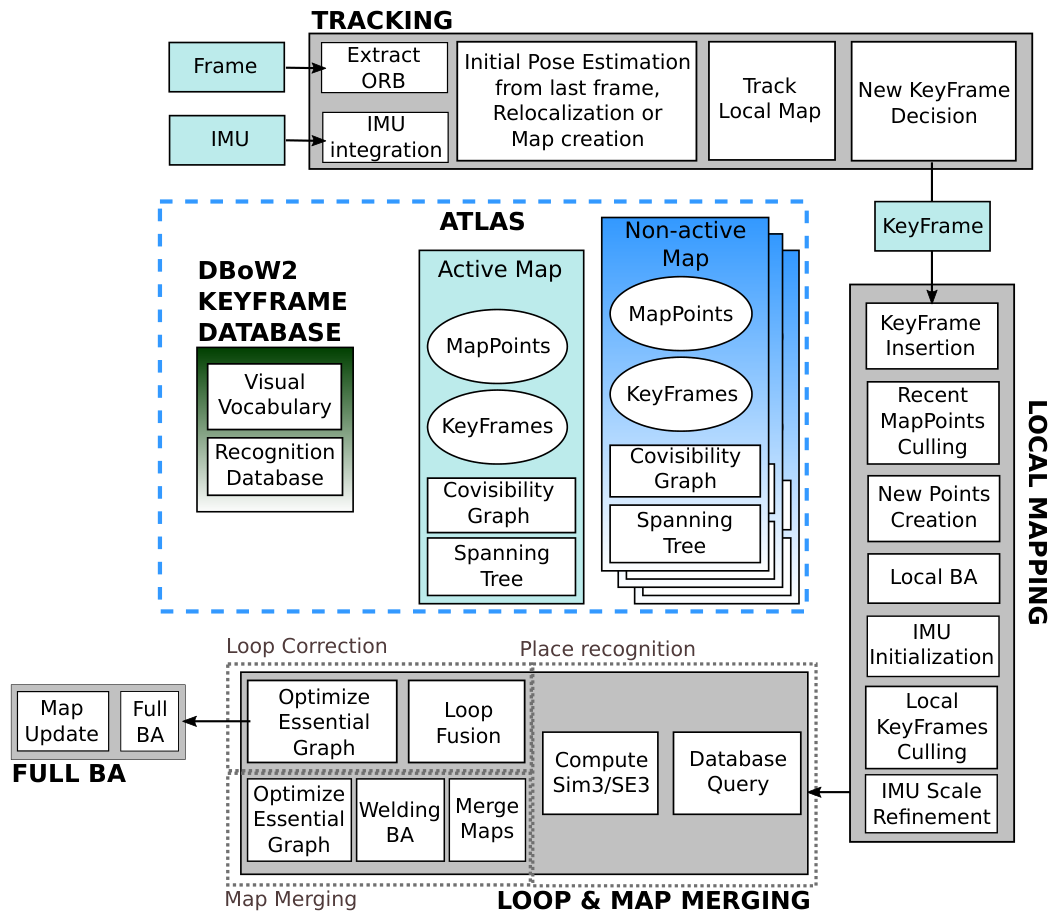
\includegraphics[width=\linewidth,height=0.50\textheight,keepaspectratio]{images/3d-vision/orbslam3_fig1_system_components.png}\\[0.2em]
      {\scriptsize Campos et al., ``ORB-SLAM3: An Accurate Open-Source Library for Visual, Visual-Inertial and Multi-Map SLAM,'' IEEE T-RO 2021, \href{https://arxiv.org/abs/2007.11898v2}{arXiv:2007.11898v2}, Figure~1.\par}
      \vspace{0.4em}
      {\scriptsize Mur-Artal et al., ``ORB-SLAM: a Versatile and Accurate Monocular SLAM System,'' IEEE T-RO 2015, \href{https://arxiv.org/abs/1502.00956v2}{arXiv:1502.00956v2}, Sec.~III and Appendix, Eqs.~8--9. Mur-Artal and Tard\'os, ``ORB-SLAM2: an Open-Source SLAM System for Monocular, Stereo and RGB-D Cameras,'' IEEE T-RO 2017, \href{https://arxiv.org/abs/1610.06475v2}{arXiv:1610.06475v2}.\par}
  \end{columns}
\end{frame}

\begin{frame}{Direct Methods: Optimizing Pixel Intensities}
  \begin{itemize}\scriptsize\itemsep0.2em
    \item \textbf{Idea:} skip descriptors; solve for the poses and depths that make high-gradient pixels agree in intensity across frames:
  \end{itemize}
  \vspace{-0.6em}
  \[ E_{\text{photo}} = \sum_{i}\,\sum_{\mathbf{p}\in\mathcal{P}_i}\,\sum_{j\in\mathrm{obs}(\mathbf{p})} \Big\lVert I_j\big(\pi(T_{ji}\,\pi^{-1}(\mathbf{p},d_{\mathbf{p}}))\big) - I_i(\mathbf{p})\Big\rVert_\gamma \]
  {\scriptsize $\mathcal{P}_i$: pixels selected in frame $i$; $\mathrm{obs}(\mathbf{p})$: frames that see $\mathbf{p}$; $d_{\mathbf{p}}=1/Z$: inverse depth; $\pi^{-1}(\mathbf{p},d_{\mathbf{p}}) = d_{\mathbf{p}}^{-1}K^{-1}\tilde{\mathbf{p}}$: back-projection; $T_{ji}=T_jT_i^{-1}$: camera $i$ to $j$; $\lVert r\rVert_\gamma$: Huber norm (robust loss), threshold $\gamma$.\par}
  \vspace{0.2em}
  \begin{columns}[T,onlytextwidth]
    \column{0.45\textwidth}
      \begin{itemize}\scriptsize\itemsep0.2em
        \item \textbf{LSD-SLAM} (large-scale direct SLAM; Engel et al., ECCV 2014): keyframes hold semi-dense inverse depth maps (only near strong gradients), refined by filtering small-baseline stereo comparisons; frames are tracked by direct alignment; Sim(3) edges in a keyframe pose graph expose scale drift. Real time on a CPU.
        \item \textbf{DSO} (direct sparse odometry; Engel et al., TPAMI 2018): 2000 active points over all gradient regions, including edges and smooth intensity variations on white walls; poses, intrinsics and inverse depths optimized jointly in a sliding window; calibrated exposure time, vignetting (darkening toward the image corners) and camera response (light reaching the sensor to pixel value).
      \end{itemize}
    \column{0.53\textwidth}
      {\centering\scriptsize\setlength{\tabcolsep}{3pt}
      \begin{tabular}{>{\raggedright\arraybackslash}p{1.45cm} >{\raggedright\arraybackslash}p{2.5cm} >{\raggedright\arraybackslash}p{2.85cm}}
        \toprule
         & \textbf{Feature-based} & \textbf{Direct} \\
        \midrule
        Usable pixels & corners with descriptors & any pixel with gradient, even in low texture \\
        \addlinespace[0.1em]
        Exposure changes & descriptors nearly invariant & modelled: calibration, per-frame affine gain and offset \\
        \addlinespace[0.1em]
        Rolling shutter & tolerated (geometric error model) & accuracy drops quickly \\
        \addlinespace[0.1em]
        Initialization & RANSAC on wide-baseline matches & needs a guess within 1--2 pixels \\
        \bottomrule
      \end{tabular}\par}
      \vspace{0.1em}
      {\scriptsize Rolling shutter: rows exposed in sequence; motion bends the image.\par}
      \vspace{0.2em}
      {\scriptsize Engel et al., ECCV 2014, \href{https://doi.org/10.1007/978-3-319-10605-2_54}{doi:10.1007/978-3-319-10605-2\_54}; TPAMI 2018, \href{https://arxiv.org/abs/1607.02565v2}{arXiv:1607.02565v2}. Cadena et al., Sec.~V.\par}
  \end{columns}
\end{frame}

\begin{frame}{Sensors, Observability, and Evaluation}
  \begin{columns}[T,onlytextwidth]
    \column{0.47\textwidth}
      \begin{itemize}\scriptsize\itemsep0.25em
        \item \textbf{Monocular:} depth, and with it scale, is not observable: trajectory and map are known up to a similarity, and the scale drifts.
        \item \textbf{Stereo and RGB-D:} the baseline $B$ or the depth sensor fixes metric scale.
        \item \textbf{Visual-inertial:} the IMU makes scale observable for a single camera; initialization also estimates the gravity direction and the IMU biases (ORB-SLAM3).
        \item \textbf{Absolute trajectory error} (ATE): align the estimated camera-to-world poses $\hat{Q}_i$ to the ground truth $Q_i$ ($\hat{Q}_i,Q_i\in SE(3)$, $i=1,\dots,n$) with the least-squares rigid transform $A$ (closed form), then
        \[ \mathrm{ATE} = \Big(\tfrac{1}{n}\textstyle\sum_{i=1}^{n}\lVert\operatorname{trans}(Q_i^{-1}A\hat{Q}_i)\rVert^2\Big)^{1/2}, \]
        the RMSE of the leftover translations. Monocular results use a 7-DoF similarity alignment, since scale is unknown.
        \item \textbf{Relative pose error} (RPE): $E_i=(Q_i^{-1}Q_{i+\Delta})^{-1}(\hat{Q}_i^{-1}\hat{Q}_{i+\Delta})$ compares the motion over a fixed interval $\Delta$, so its RMSE measures drift ($\Delta=30$ frames at 30\,Hz gives drift per second).
      \end{itemize}
    \column{0.51\textwidth}
      \vspace{0.2em}
      {\centering\scriptsize\setlength{\tabcolsep}{3pt}
      \begin{tabular}{>{\raggedright\arraybackslash}p{1.5cm} >{\raggedright\arraybackslash}p{2.8cm} >{\raggedright\arraybackslash}p{2.2cm}}
        \toprule
        \textbf{Benchmark} & \textbf{Sensors and platform} & \textbf{Ground truth} \\
        \midrule
        TUM RGB-D (Sturm et al., 2012) & Kinect RGB-D, $640\times480$ at 30\,Hz, hand-held or on a robot; 39 indoor sequences & motion capture, 8 cameras at 100\,Hz \\
        \addlinespace[0.2em]
        EuRoC MAV (Burri et al., 2016) & stereo and IMU on a micro aerial vehicle; 11 flights, from slow to fast with motion blur & laser tracker (mm position) or motion capture (6-DoF pose) \\
        \addlinespace[0.2em]
        KITTI odometry (Geiger et al., 2012) & stereo cameras at 10\,Hz on a car; 22 sequences, 39.2\,km & GPS/IMU with real-time kinematic (RTK) correction \\
        \bottomrule
      \end{tabular}\par}
      \vspace{0.5em}
      {\scriptsize Sturm et al., ``A Benchmark for the Evaluation of RGB-D SLAM Systems,'' IROS 2012, \href{https://doi.org/10.1109/IROS.2012.6385773}{doi:10.1109/IROS.2012.6385773}, Sec.~VII. Burri et al., ``The EuRoC Micro Aerial Vehicle Datasets,'' IJRR 2016, \href{https://doi.org/10.1177/0278364915620033}{doi:10.1177/0278364915620033}. Geiger et al., ``Are We Ready for Autonomous Driving? The KITTI Vision Benchmark Suite,'' CVPR 2012, \href{https://doi.org/10.1109/CVPR.2012.6248074}{doi:10.1109/CVPR.2012.6248074}. Campos et al., \href{https://arxiv.org/abs/2007.11898v2}{arXiv:2007.11898v2}, Sec.~II-B and V-B.\par}
  \end{columns}
\end{frame}

\begin{frame}{Learned SLAM: DROID-SLAM}
  \centering
  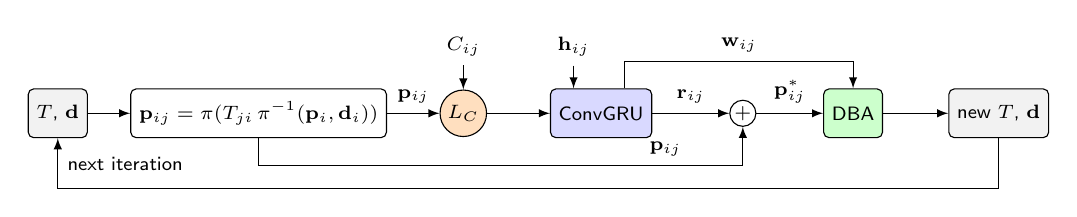
\begin{tikzpicture}[font=\sffamily\scriptsize, >=latex,
      op/.style={draw, rounded corners=2pt, align=center, inner sep=3pt, minimum height=0.62cm},
      lk/.style={draw, circle, fill=orange!25, inner sep=1.5pt},
      sm/.style={draw, circle, inner sep=0.5pt}]
    \node[op, fill=gray!10] (Td) at (0,0) {$T$, $\mathbf{d}$};
    \node[op] (proj) at (2.55,0) {$\mathbf{p}_{ij}=\pi(T_{ji}\,\pi^{-1}(\mathbf{p}_i,\mathbf{d}_i))$};
    \node[lk] (L) at (5.15,0) {$L_C$};
    \node[op, fill=blue!15] (gru) at (6.9,0) {ConvGRU};
    \node[sm] (plus) at (8.7,0) {$+$};
    \node[op, fill=green!20] (dba) at (10.1,0) {DBA};
    \node[op, fill=gray!10] (Tn) at (11.95,0) {new $T$, $\mathbf{d}$};
    \node (C) at (5.15,0.85) {$C_{ij}$};
    \node (h) at (6.55,0.85) {$\mathbf{h}_{ij}$};
    \draw[->] (Td) -- (proj);
    \draw[->] (proj) -- node[above] {$\mathbf{p}_{ij}$} (L);
    \draw[->] (C) -- (L);
    \draw[->] (L) -- (gru);
    \draw[->] (h) -- (h |- gru.north);
    \draw[->] (gru) -- node[above] {$\mathbf{r}_{ij}$} (plus);
    \draw[->] (proj.south) -- ++(0,-0.35) -| node[pos=0.42, above] {$\mathbf{p}_{ij}$} (plus.south);
    \draw[->] (plus) -- node[above] {$\mathbf{p}^*_{ij}$} (dba);
    \draw[->] ([xshift=0.3cm]gru.north) -- ++(0,0.34) -| node[pos=0.25, above] {$\mathbf{w}_{ij}$} (dba.north);
    \draw[->] (dba) -- (Tn);
    \draw[->] (Tn.south) -- ++(0,-0.64) -| node[pos=0.75, right] {next iteration} (Td.south);
  \end{tikzpicture}\\[0.1em]
  {\scriptsize One iteration of the update operator for one edge $(i,j)$; it runs on every edge of the frame graph. After Teed and Deng, ``DROID-SLAM: Deep Visual SLAM for Monocular, Stereo, and RGB-D Cameras,'' NeurIPS 2021, \href{https://arxiv.org/abs/2108.10869v2}{arXiv:2108.10869v2}, Figure~2.\par}
  \vspace{0.3em}
  \begin{columns}[T,onlytextwidth]
    \column{0.50\textwidth}
      \begin{itemize}\scriptsize\itemsep0.25em
        \item \textbf{State:} a pose $T_t\in SE(3)$ and a dense inverse-depth map $\mathbf{d}_t$ per frame. A frame graph links covisible frames; edges to old frames are added when the camera returns, which closes loops.
        \item \textbf{Update operator} (above): $\mathbf{p}_i$ is the pixel grid of frame $i$ and $T_{ji}=T_jT_i^{-1}$. A lookup $L_C$ in the correlation volume $C_{ij}$ around $\mathbf{p}_{ij}$ and a $3\times3$ convolutional GRU with hidden state $\mathbf{h}_{ij}$ (both as in RAFT) predict a flow revision $\mathbf{r}_{ij}$ and a confidence $\mathbf{w}_{ij}$.
        \item \textbf{Beyond RAFT:} RAFT revises the flow between two frames; here the updates act on any number of frames, and a dense bundle adjustment (DBA) layer refines all poses and depth maps jointly, which the authors call essential for low drift on long trajectories and for loop closure.
      \end{itemize}
    \column{0.48\textwidth}
      \begin{itemize}\scriptsize\itemsep0.25em
        \item \textbf{DBA layer:} Gauss--Newton steps on all poses and depths, solved with the Schur complement, toward the revised targets $\mathbf{p}^*_{ij}=\mathbf{p}_{ij}+\mathbf{r}_{ij}$:
        \[ E(T',\mathbf{d}')=\sum_{(i,j)\in\mathcal{E}}\mathbf{e}_{ij}^\top\,\mathrm{diag}(\mathbf{w}_{ij})\,\mathbf{e}_{ij} \]
        with $\mathbf{e}_{ij}=\mathbf{p}^*_{ij}-\pi(T'_{ji}\,\pi^{-1}(\mathbf{p}_i,\mathbf{d}'_i))$. The confidences act as the information matrix ($\Lambda_{ij}$), so confident pixels count more.
        \item The layer is part of the computation graph, so training backpropagates through it end to end.
      \end{itemize}
  \end{columns}
\end{frame}

\begin{frame}{DROID-SLAM: Training and Results}
  \begin{columns}[T,onlytextwidth]
    \column{0.48\textwidth}
      \begin{itemize}\scriptsize\itemsep0.3em
        \item \textbf{Data:} one model, trained only on monocular video from the synthetic TartanAir dataset (photo-realistic simulation), in 7-frame clips whose neighbouring frames move 8 to 96 pixels on average.
        \item \textbf{Loss:} a pose loss (distance between predicted and true poses) plus a flow loss (flow induced by the predicted against the true poses and depths), applied to all 15 unrolled iterations with weights growing toward the last ($\gamma=0.9$). 250k steps, batch 4, $384\times512$ images: one week on four RTX 3090 GPUs.
        \item \textbf{Gauge:} in training the first two poses are fixed to ground truth: the first removes the 6-DoF gauge freedom, the second the scale.
        \item \textbf{Inference:} a front-end thread adds keyframes and runs local BA; a back-end thread runs global BA over all keyframes. Stereo uses both images with the left-right pose fixed; RGB-D adds a term on the measured depth. Real time needs two RTX 3090 GPUs.
      \end{itemize}
    \column{0.50\textwidth}
      \centering
      {\scriptsize TUM RGB-D fr1 (the 9 office sequences), RGB input only:\par}
      \vspace{0.2em}
      {\scriptsize\setlength{\tabcolsep}{4pt}
      \begin{tabular}{l c c}
        \toprule
        \textbf{Method} & \textbf{Tracked} & \textbf{Mean ATE (m)} \\
        \midrule
        ORB-SLAM2 & 3 of 9 & lost on 6 \\
        ORB-SLAM3 & 4 of 9 & lost on 5 \\
        DeepFactors & 9 of 9 & 0.233 \\
        DROID-SLAM & 9 of 9 & \textbf{0.038} \\
        \bottomrule
      \end{tabular}\par}
      \vspace{0.2em}
      {\scriptsize DeepFactors is a learned dense monocular SLAM system. Two baselines given extra information reach 0.116\,m (RGB-D input) and 0.206\,m (ground-truth scale).\par}
      \vspace{0.3em}
      \begin{itemize}\scriptsize\itemsep0.25em
        \item \textbf{EuRoC, monocular} (11 flights): 0.022\,m mean ATE against 0.126\,m for the best method without failures (82\% lower); 43\% lower than ORB-SLAM3 on the 10 flights it completes.
        \item \textbf{TartanAir test:} competition error 62\% (mono) and 60\% (stereo) lower than the best prior entry, while running 16 times faster.
      \end{itemize}
      \vspace{0.2em}
      {\scriptsize Teed and Deng, \href{https://arxiv.org/abs/2108.10869v2}{arXiv:2108.10869v2}, Sec.~3.3--4, Tables~2--4. Czarnowski et al., ``DeepFactors: Real-Time Probabilistic Dense Monocular SLAM,'' IEEE RA-L 2020, \href{https://arxiv.org/abs/2001.05049v1}{arXiv:2001.05049v1}. Wang et al., ``TartanAir: A Dataset to Push the Limits of Visual SLAM,'' IROS 2020, \href{https://arxiv.org/abs/2003.14338v2}{arXiv:2003.14338v2}.\par}
  \end{columns}
\end{frame}

\begin{frame}{Dense Maps: TSDF Fusion}
  \begin{columns}[T,onlytextwidth]
    \column{0.55\textwidth}
      \begin{itemize}\scriptsize\itemsep0.12em
        \item \textbf{Truncated signed distance function (TSDF)} (KinectFusion, Newcombe et al., ISMAR 2011): each voxel (3D grid cell) $\mathbf{p}$ stores the signed distance $F(\mathbf{p})$ to the nearest surface, positive in front and negative behind, truncated at $\pm\mu$, and a weight $W(\mathbf{p})$.
        \item \textbf{Fusion:} depth map $D_k$ gives a TSDF $F_{D_k}$ with weights $W_{D_k}$ (distances measured along each pixel's ray), averaged into the volume:
        \[ F_k=\frac{W_{k-1}F_{k-1}+W_{D_k}F_{D_k}}{W_{k-1}+W_{D_k}},\qquad W_k=W_{k-1}+W_{D_k} \]
        Setting $W_{D_k}=1$ gives a plain average, which the authors found works well.
        \item \textbf{Surface and tracking:} the surface is the zero crossing of $F$. Raycasting (each pixel's ray marched to the zero crossing) predicts the surface seen from the last pose; the new depth frame is aligned to it by ICP (iterative closest point): each new point is paired with the predicted surface point it projects to, the pose that minimizes their distances along the surface normals (point-to-plane) is solved for, and the two steps repeat, coarse to fine, in real time on a GPU. Tracking against the fused model drifts less than frame-to-frame tracking.
        \item Cadena et al.\ (Sec.~V) note that TSDFs became a popular map for vision-based SLAM after KinectFusion.
      \end{itemize}
    \column{0.43\textwidth}
      \centering
      \vspace{0.6em}
      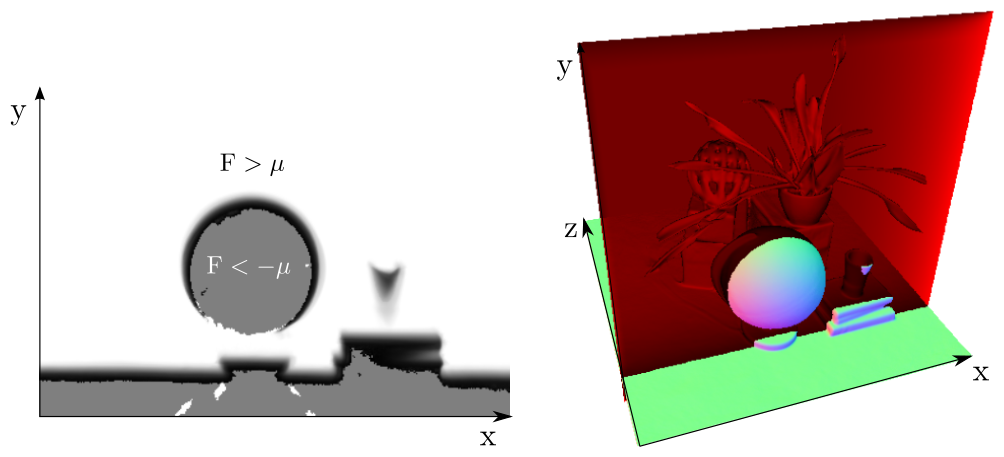
\includegraphics[width=\linewidth,height=0.45\textheight,keepaspectratio]{images/3d-vision/kinectfusion_fig4_tsdf_slice.png}\\[0.2em]
      {\scriptsize Left: a slice through the volume, with truncated free space $F>\mu$ (white), the smooth distance field around the surface $F=0$, and voxels without a valid measurement yet (grey). Right: the scene, with the slice plane in red. Newcombe et al., ``KinectFusion: Real-Time Dense Surface Mapping and Tracking,'' ISMAR 2011, \href{https://doi.org/10.1109/ISMAR.2011.6092378}{doi:10.1109/ISMAR.2011.6092378}, Figure~4.\par}
  \end{columns}
\end{frame}

\begin{frame}{Dense Maps: Gaussian Splatting SLAM}
  \begin{columns}[T,onlytextwidth]
    \column{0.49\textwidth}
      \begin{itemize}\scriptsize\itemsep0.25em
        \item \textbf{NeRF} (neural radiance field; Mildenhall et al., ECCV 2020): an MLP maps a 3D position and viewing direction to density and colour; volume rendering sums the colours along each camera ray, weighted by density and by the transparency in front.
        \item \textbf{3D Gaussian splatting} (Kerbl et al., ACM TOG 2023): the scene is a set of anisotropic 3D Gaussians (stretched differently along each axis), each with a mean, covariance $\Sigma=R\,\mathrm{diag}(\mathbf{s})^2R^\top$ ($R$ stored as a quaternion; $\mathbf{s}$ the 3D scale vector), opacity $\alpha$, and view-dependent colour from spherical harmonics (a basis of functions on the sphere). A differentiable tile-based rasterizer projects each Gaussian to a 2D ellipse, sorts them by depth and alpha-blends them front to back, at 30\,fps or more at 1080p.
      \end{itemize}
    \column{0.49\textwidth}
      \begin{itemize}\scriptsize\itemsep0.25em
        \item \textbf{Gaussian Splatting SLAM} (Matsuki et al., CVPR 2024): the first monocular SLAM system with Gaussians as its only map.
        \item \textbf{Tracking:} only the camera pose $T_{CW}$ is optimized, to minimize $\lVert I(\mathcal{G},T_{CW})-\bar{I}\rVert_1$, the L1 difference between the rendered Gaussians $\mathcal{G}$ and the frame $\bar{I}$, using analytic Jacobians of the rendering with respect to the pose.
        \item \textbf{Mapping:} the Gaussians and the poses of a window of keyframes are optimized together; a regularizer pushes Gaussians toward isotropy, because rendering does not constrain their extent along the viewing ray.
        \item Runs live at 3\,fps; with a depth sensor it adds a depth residual.
      \end{itemize}
  \end{columns}
  \vspace{0.2em}
  \centering
  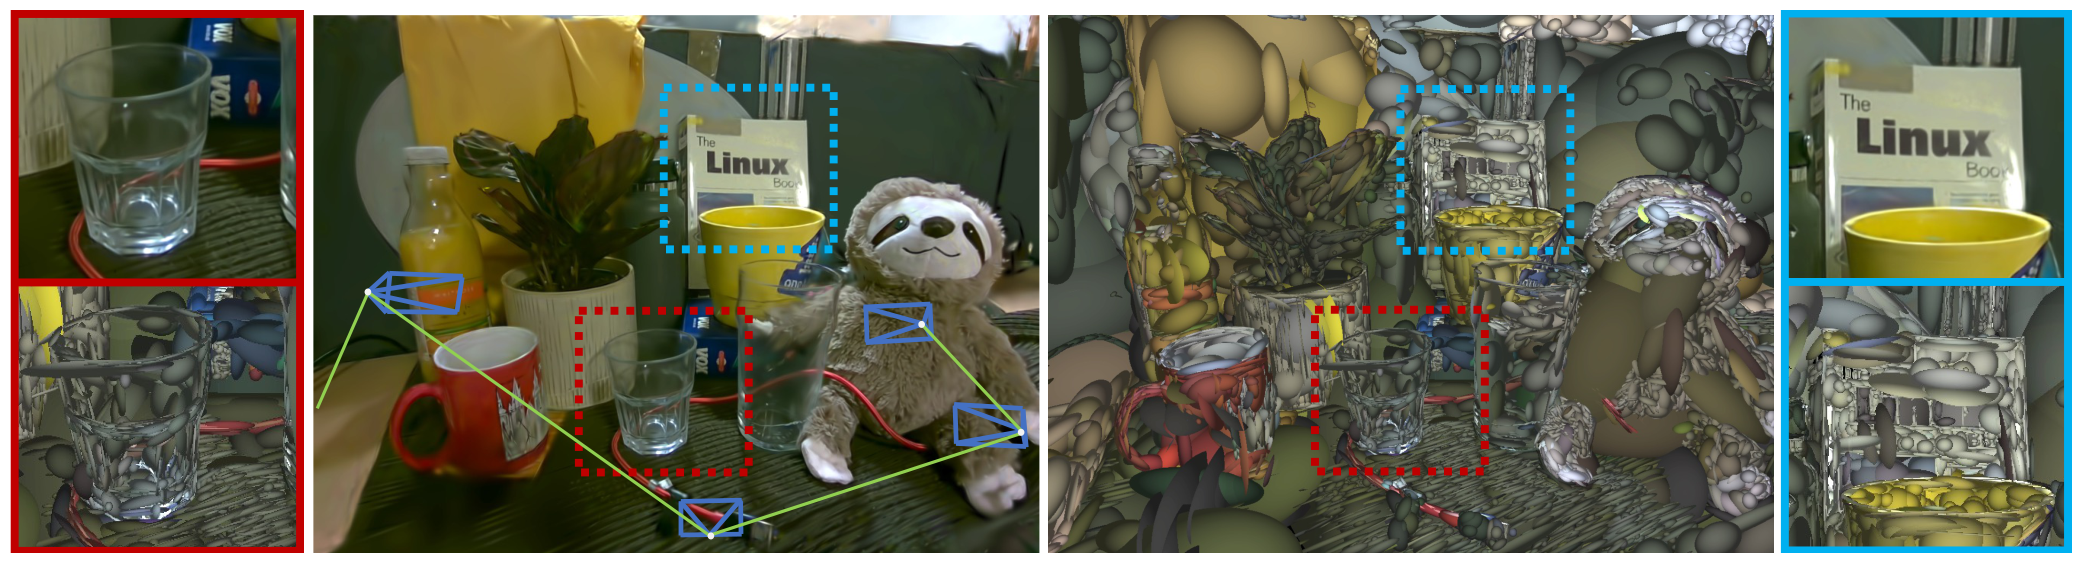
\includegraphics[width=\textwidth,height=0.24\textheight,keepaspectratio]{images/3d-vision/gsslam_fig1_monocular_gaussian_map.png}\\[0.2em]
  {\scriptsize Center: rasterised Gaussians with camera poses, then shaded; sides: dotted-box close-ups (top rasterised, bottom shaded).\\ Matsuki et al., ``Gaussian Splatting SLAM,'' CVPR 2024, \href{https://arxiv.org/abs/2312.06741v2}{arXiv:2312.06741v2}, Figure~1.\par}
\end{frame}
